%
% $Id: $
%
%
% Compilar a .pdf con LaTeX (pdflatex)
% Es necesario instalar Beamer (paquete latex-beamer en Debian)
%

%
% Gr�ficos:
% Los gr�ficos pueden suministrarse en PNG, JPG, TIF, PDF, MPS
% Los EPS deben convertirse a PDF (usar epstopdf)
%

\documentclass{beamer}
\usetheme{Warsaw}
%\usebackgroundtemplate{
\includegraphics[width=\paperwidth]{format/libresoft-bg.png}}
%\usepackage[spanish]{babel}
\usepackage[latin1]{inputenc}
\usepackage{graphics}
\usepackage{amssymb} % Simbolos matematicos
\usepackage{url}

%\definecolor{libresoftgreen}{RGB}{162,190,43}
%\definecolor{libresoftblue}{RGB}{0,98,143}

%\setbeamercolor{titlelike}{bg=libresoftgreen}

%% Metadatos del PDF.
\hypersetup{
  pdftitle={Automatic analysis of Scratch projects to assess computational thinking skills},
  pdfauthor={Jes�s Moreno Le�n, Gregorio Robles},
  pdfcreator={GSyC/LibreSoft \\ Universidad Rey Juan Carlos},
  pdfproducer=PDFLaTeX,
  pdfsubject={Computational Thinking. Automatic assessment with Dr. Scratch.},
}
%%

\begin{document}

\title{Automatic analysis of Scratch projects to assess computational thinking skills}
\institute{jesus.moreno@programamos.es, grex@gsyc.urjc.es \\
GSyC/Libresoft, Universidad Rey Juan Carlos}
\author{Jes�s Moreno Le�n, Gregorio Robles}
\date{Computational Thinking and Coding at Schools \\ Vienna. April 18, 2016}

\frame{
\maketitle
\begin{center}

\includegraphics[width=2cm]{format/libresoft-logo}
\hspace{0.5cm}

\includegraphics[width=5cm]{format/gsyc-urjc}
\vspace{0.5cm}

\includegraphics[width=3cm]{format/emadrid.png}
\end{center}
}


% Si el titulo o el autor se quieren acortar para los pies de p�gina
% se pueden redefinir aqu�:
\title{Automatic analysis of Scratch projects to assess CT skills}
%\author{Autores abreviado}

%% LICENCIA DE REDISTRIBUCION DE LAS TRANSPAS
\frame{
~
\vspace{3cm}

\begin{flushright}

\includegraphics[width=2.2cm]{figs/by-sa}

{\tiny
(cc) 2016 Jes�s Moreno Le�n and Gregorio Robles\\
  Some rights reserved. This work licensed under Creative Commons \\
  Attribution-ShareAlike License. To view a copy of full license, see \\
  http://creativecommons.org/licenses/by-sa/3.0/ or write to \\
  Creative Commons, 559 Nathan Abbott Way, Stanford, \\
  California 94305, USA. \\
\ \\
Some of the figures have been taken from the Internet \\
Source, and author and licence if known, is specified. \\
For those images, \emph{fair use} applies.
}
\end{flushright}
}
%%

\section{Scratch Conference 2015, Amsterdam}


%--------------------------------------------------------
%\usebackgroundtemplate{
\includegraphics[width=10cm]{figs/drscratch1}}

\begin{frame}
\frametitle{What is Dr. Scratch?}

\begin{figure}[t!]
\begin{center}

\includegraphics[width=9cm]{figs/drscratch1.png}
\end{center}
\label{fig:naming}
\end{figure}

\end{frame}

%--------------------------------------------------------
%\usebackgroundtemplate{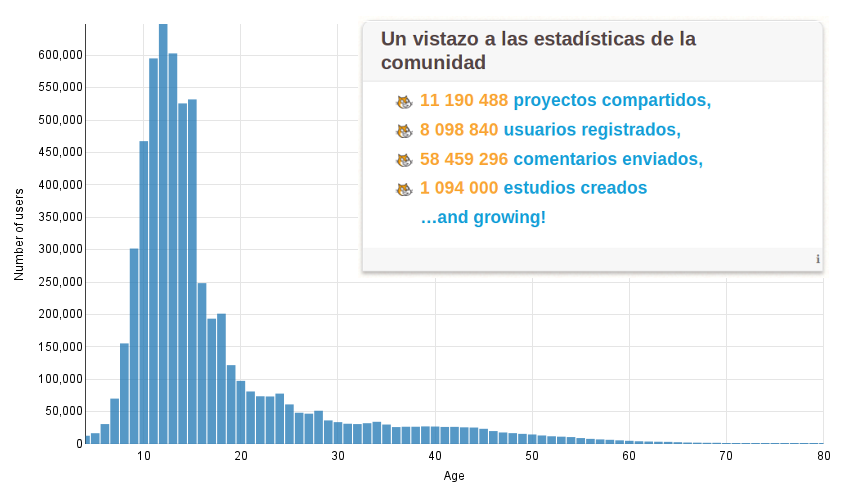
\includegraphics[width=18cm]{figs/stats.png}}

\begin{frame}
\frametitle{Remixing other researchers' ideas}
\begin{columns}[T]
    \begin{column}{1\textwidth}
     \begin{block}{Analysis of Scratch projects}
       \begin{itemize}
	 \item \texttt{Scrape}: visual representation of the blocks used (and not used).
         \item \texttt{Hairball}: static analyzer of Scratch projects to detect errors.
         \item Brennan \& Resnick: New frameworks for studying and assessing the development of CT.
         \item Seiter \& Foreman: Progression of Early CT Model.
         \item Wilson, Hainey \& Connolly: Evaluation of games to gauge understanding of programming concepts.
         %\item Koh, Basawapatna, Bennett, \& Repenning: Towards the Automatic Recognition of Computational Thinking for Adaptive Visual Language Learning
       \end{itemize}
    \end{block}
    \end{column}
  \end{columns}
\end{frame}

\usebackgroundtemplate{}

%--------------------------------------------------------
%\usebackgroundtemplate{\includegraphics[width=13cm]{figs/iceberg.jpg}}
% background: http://www.wim-network.org/wp-content/uploads/2012/04/iceberg.jpg

\begin{frame}
\frametitle{Assessment of CT development}
\begin{table}[t]\tiny 
\centering
%\begin{tabular}{p{2.5cm}p{2.7cm}p{3cm}p{4cm}}
\begin{tabular}{|p{2cm}|p{2cm}|p{2cm}|p{2cm}|}
%\toprule
\hline
CT aspect & Basic & Developing & Proficient\\ %\midrule 
\hline
\hline  
Data representation & modifiers of sprites properties &
operations on vars & operations on lists  \\
\hline
Logical Thinking & if & if else & logic operations \\ 
\hline
User interactivity & green flag & key pressed, sprite clicked, ask and wait,
mouse blocks & when \%s is \textgreater \%s, video, audio \\ 
\hline
Algotithmic notions of flow control & sequence of blocks & repeat, forever & repeat until \\ 
\hline
Abstraction and problem decomposition & more than one script and more than one sprite & def block & when I start as clone\\
\hline
Parallelism & Two scripts on green flag & Two scripts on key pressed, two scripts on sprite clicked on the same sprite & Two scripts on when I receive message, two scripts when \%s is \textgreater \%s, two scripts on when backdrop change to \\
\hline
Synchronization & wait & Broadcast, when I receive message, stop all, stop program, stop programs sprite & wait until, when backdrop change to, broadcast and wait \\ 
\hline
\end{tabular}
\caption{Level of development for each CT dimension}
\label{table:CTscore}
\end{table}

\end{frame}

%--------------------------------------------------------
\begin{frame}
\frametitle{Assessment of CT development: Logical Thinking}

\begin{figure}[t!]
\begin{center}
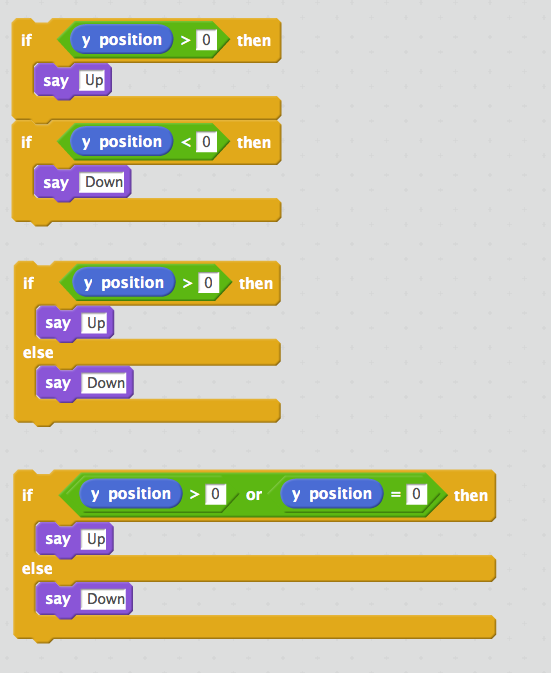
\includegraphics[height=6cm]{figs/Logic.png}
\end{center}
\label{fig:logic}
\end{figure}

\begin{center}
Different levels of development of logical thinking: basic (top), developing (center) and proficient (bottom).
\end{center}
\end{frame}

%--------------------------------------------------------
\begin{frame}
\frametitle{Assessment of CT development: Data Representation}

\begin{figure}[t!]
\begin{center}
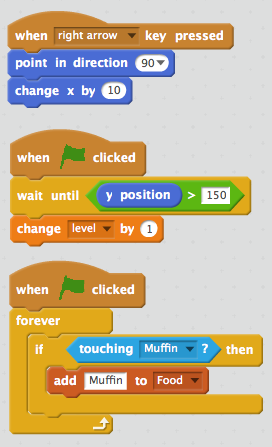
\includegraphics[height=6cm]{figs/Data.png}
\end{center}
\label{fig:logic}
\end{figure}

\begin{center}
Different levels of development of data representation: basic (top), developing (center) and proficient (bottom).
\end{center}
\end{frame}

%--------------------------------------------------------
\usebackgroundtemplate{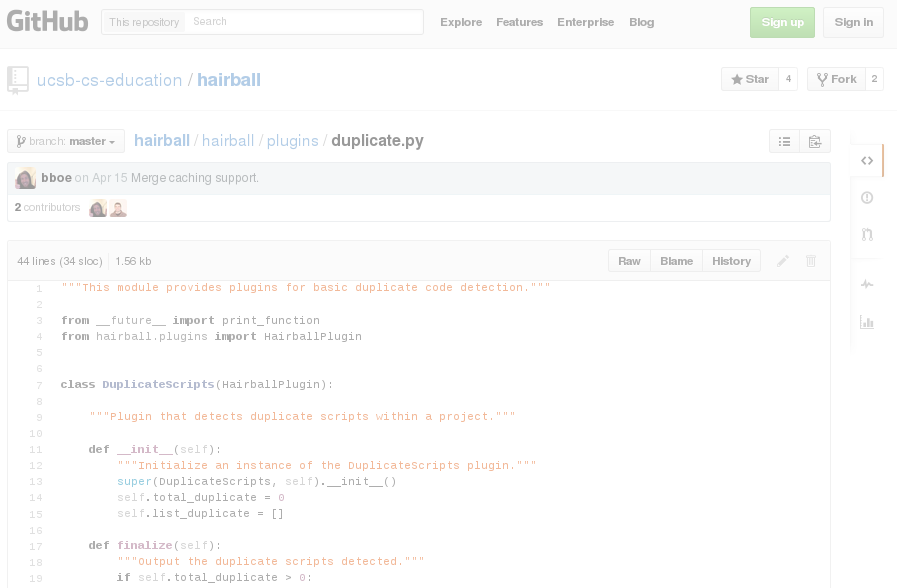
\includegraphics[width=13cm,height=9.2cm]{figs/plugins.png}}
\begin{frame}
\frametitle{Code smells (I)}
\begin{columns}[T]
    \begin{column}{0.8\textwidth}
     \begin{block}{Errors or bad programming habits}
\begin{itemize}
  \item Dead code
  \item Attribute initialization
  \item Default names
  \item Repeated scripts
\end{itemize}
    \end{block}
    \end{column}
  \end{columns}
\end{frame}

\usebackgroundtemplate{}
%--------------------------------------------------------
\begin{frame}
\frametitle{Code smells (II)}

\begin{figure}[t!]
\begin{center}
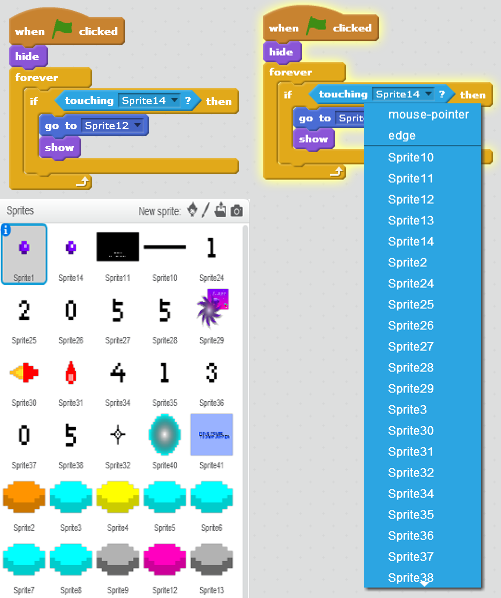
\includegraphics[width=7cm, height=6cm]{figs/SpriteNaming.png}
\end{center}
\label{fig:naming}
\end{figure}

\begin{center}
\emph{Bad}/default naming of sprites
\end{center}
\end{frame}

\usebackgroundtemplate{}
%--------------------------------------------------------

\begin{frame}
\frametitle{Code smells (and III)}

  \begin{columns}[T]
    \begin{column}{0.5\textwidth}
 
     \begin{block}{Example of repeated code}
\begin{figure}[t!]
\begin{center}
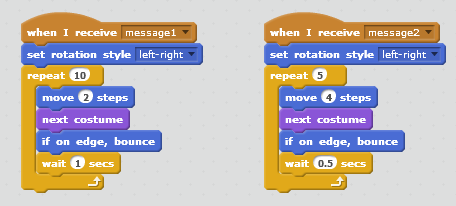
\includegraphics[width=5.4cm,height=2.5cm]{figs/CodeRepetition1.png}
\end{center}
\label{fig:repetition1}
\end{figure}
     \end{block}
    \end{column}
    \begin{column}{0.5\textwidth}
     \begin{block}{Solution to avoid repeated code}
\begin{figure}[t!]
\begin{center}
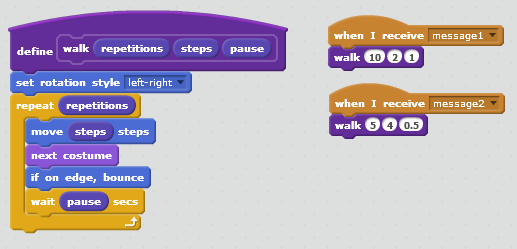
\includegraphics[width=5.4cm,height=2.5cm]{figs/CodeRepetition2.png}
\end{center}
Blocks should be created to avoid repetition of code
\label{fig:repetition2}
\end{figure}
     \end{block}

    \end{column}
  \end{columns}

\end{frame}

\usebackgroundtemplate{}

%--------------------------------------------------------
\begin{frame}
\frametitle{Dr. Scratch vs Expert judgement}
\begin{center}
Imagen del concurso Dr. Scratch
\end{center}
\end{frame}

\usebackgroundtemplate{}

%--------------------------------------------------------
\begin{frame}
\frametitle{Dr. Scratch vs Expert judgement (and II)}
\begin{center}
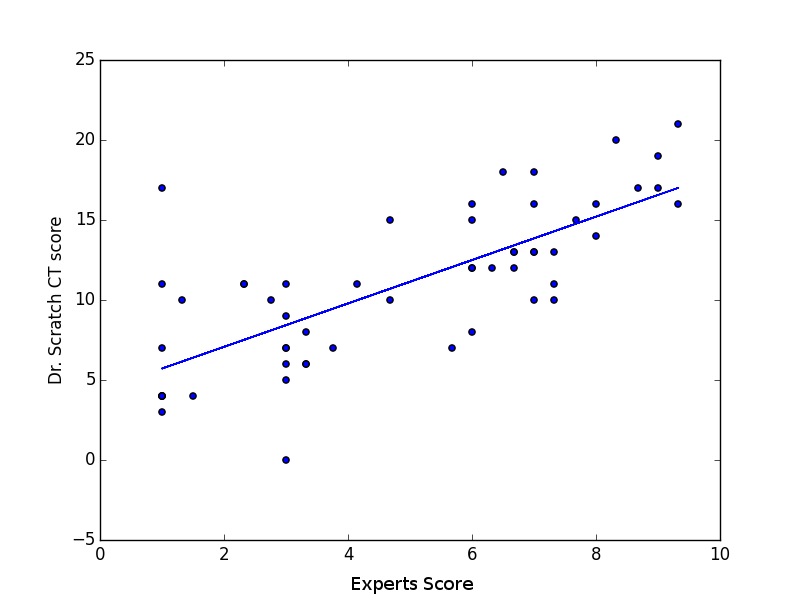
\includegraphics[height=6cm]{figs/experts.png}
\end{center}
\end{frame}

\usebackgroundtemplate{}

%--------------------------------------------------------
\begin{frame}
\frametitle{Dr. Scratch vs other CT assessment tools}
\begin{center}
\end{center}
\end{frame}

\usebackgroundtemplate{}

%--------------------------------------------------------
\begin{frame}
\frametitle{Dr. Scratch vs classic software engineering complexity metrics (I)}
\begin{center}
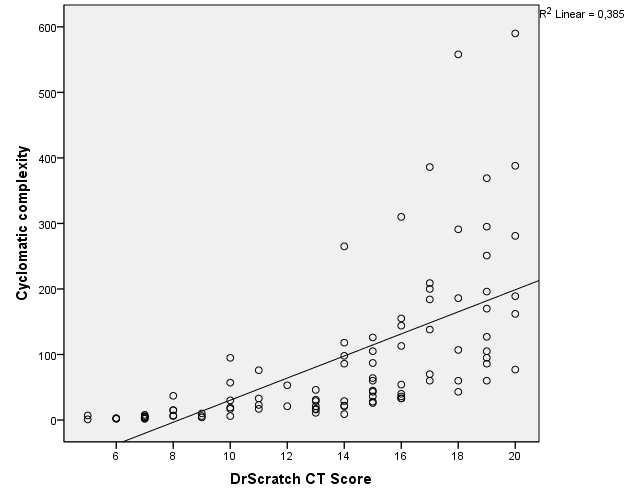
\includegraphics[height=6cm]{figs/CC.png}
\end{center}
\end{frame}

\usebackgroundtemplate{}

%--------------------------------------------------------
\begin{frame}
\frametitle{Dr. Scratch vs classic software engineering complexity metrics (II)}
\begin{center}
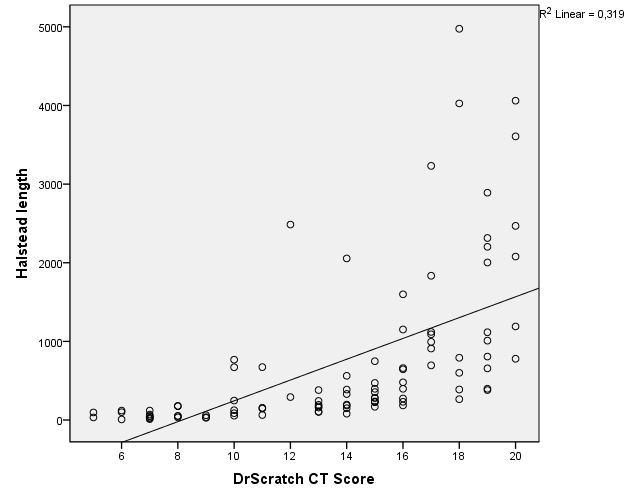
\includegraphics[height=6cm]{figs/length.png}
\end{center}
\end{frame}

\usebackgroundtemplate{}

%--------------------------------------------------------
\begin{frame}
\frametitle{Dr. Scratch vs classic software engineering complexity metrics (and III)}
\begin{center}
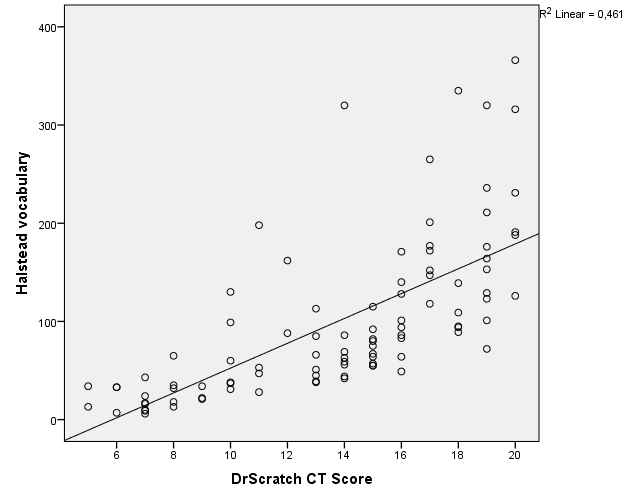
\includegraphics[height=6cm]{figs/vocabulary.png}
\end{center}
\end{frame}

\usebackgroundtemplate{}

%--------------------------------------------------------
\begin{frame}
\frametitle{Does Dr. Scratch foster CT skills? (I)}
\begin{center}
\begin{center}
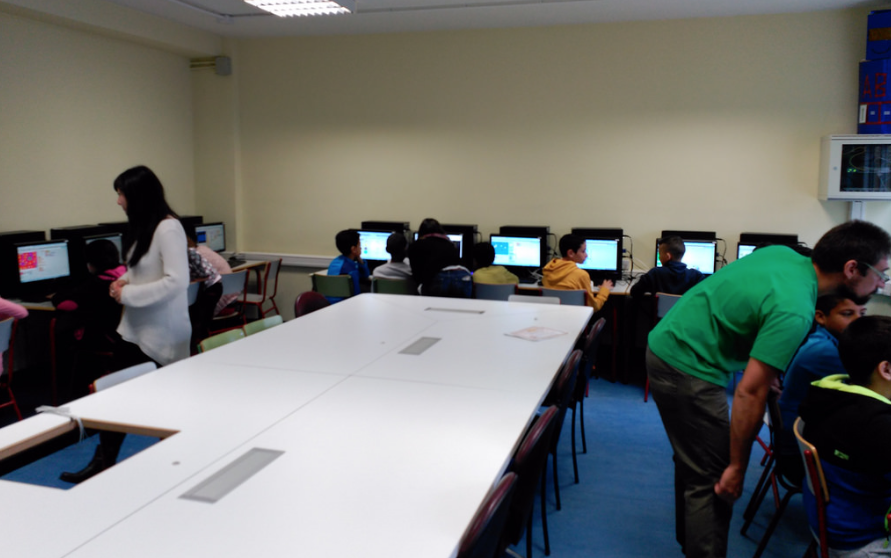
\includegraphics[height=6cm]{figs/colegio.png}
\end{center}
Workshop at CEIP Lope de Vega, Madrid (Spain)
\end{center}
\end{frame}

\usebackgroundtemplate{}

%--------------------------------------------------------
\begin{frame}
\frametitle{Does Dr. Scratch foster CT skills? (II)}
\begin{center}
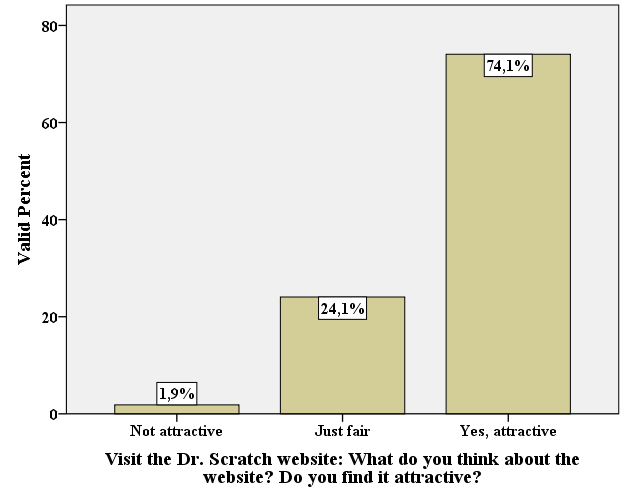
\includegraphics[height=6cm]{figs/attractive.png}
\end{center}
\end{frame}

\usebackgroundtemplate{}

%--------------------------------------------------------
\begin{frame}
\frametitle{Does Dr. Scratch foster CT skills? (III)}
\begin{center}
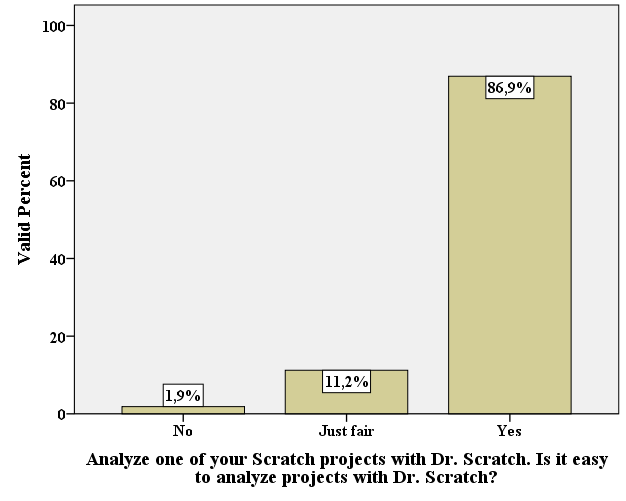
\includegraphics[height=6cm]{figs/easy.png}
\end{center}
\end{frame}

\usebackgroundtemplate{}

%--------------------------------------------------------
\begin{frame}
\frametitle{Does Dr. Scratch foster CT skills? (IV)}
\begin{center}
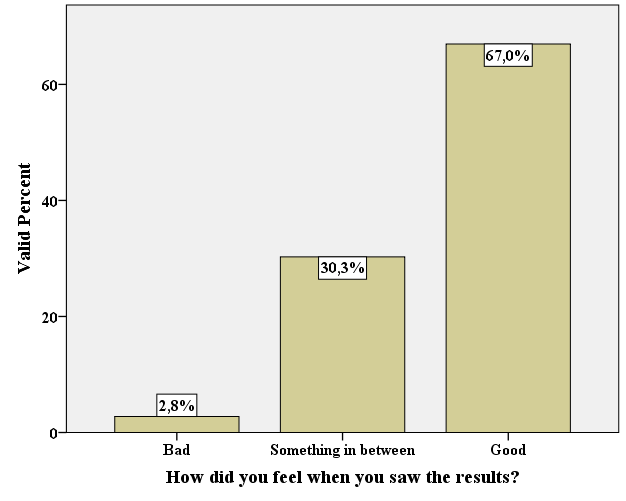
\includegraphics[height=6cm]{figs/feeling.png}
\end{center}
\end{frame}

\usebackgroundtemplate{}

%--------------------------------------------------------
\begin{frame}
\frametitle{Does Dr. Scratch foster CT skills? (V)}
\begin{center}
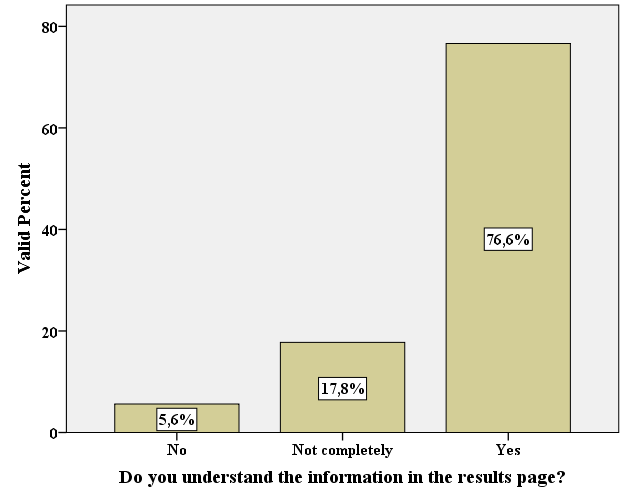
\includegraphics[height=6cm]{figs/understand.png}
\end{center}
\end{frame}

\usebackgroundtemplate{}

%--------------------------------------------------------
\begin{frame}
\frametitle{Does Dr. Scratch foster CT skills? (and VI)}
\begin{center}
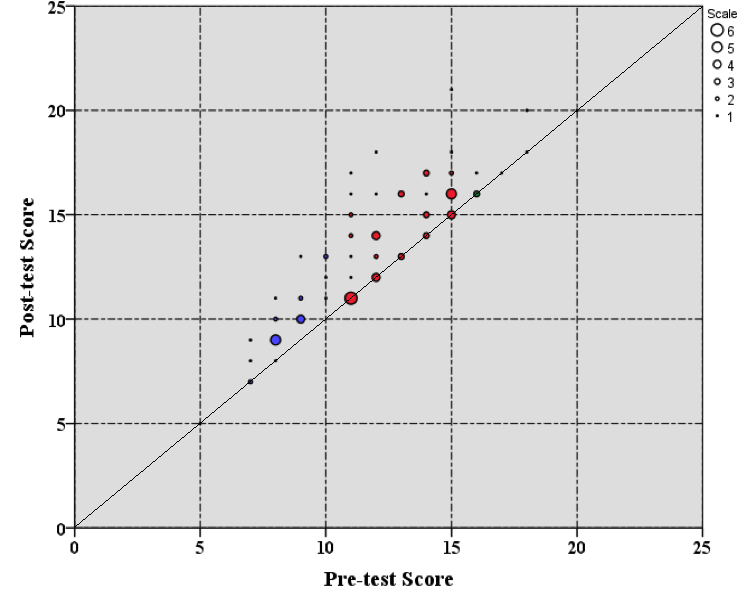
\includegraphics[height=6cm]{figs/improvement.png}
\end{center}
\end{frame}

\usebackgroundtemplate{}

%--------------------------------------------------------
\begin{frame}
\frametitle{Teachers' testimonials}
\begin{center}
\end{center}
\end{frame}

\usebackgroundtemplate{}

%--------------------------------------------------------
%\usebackgroundtemplate{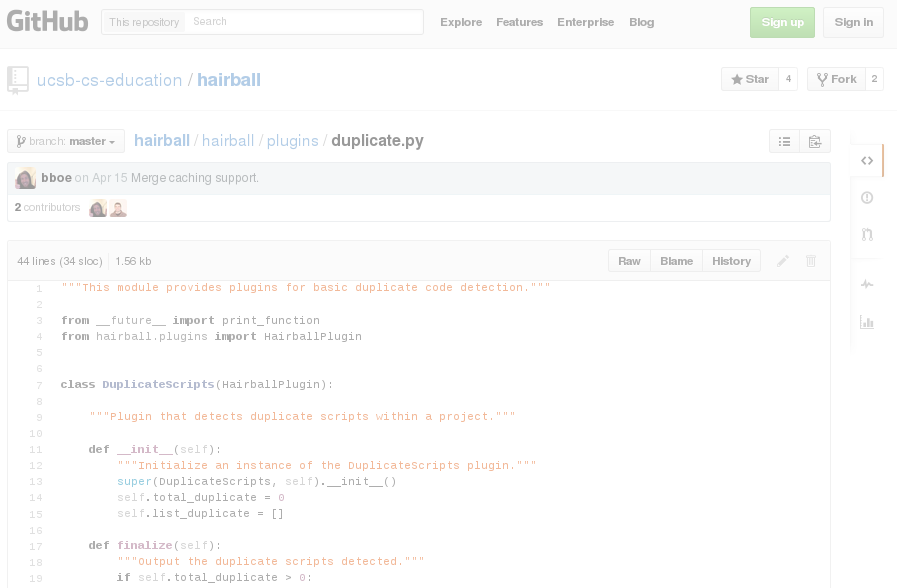
\includegraphics[width=13cm,height=9.2cm]{figs/plugins.png}}
% background: http://25.media.tumblr.com/b83aa72682992ab34b8ce7e61c0cb7f9/tumblr_menxc7qcq61ryin08o1_r1_1280.jpg
\usebackgroundtemplate{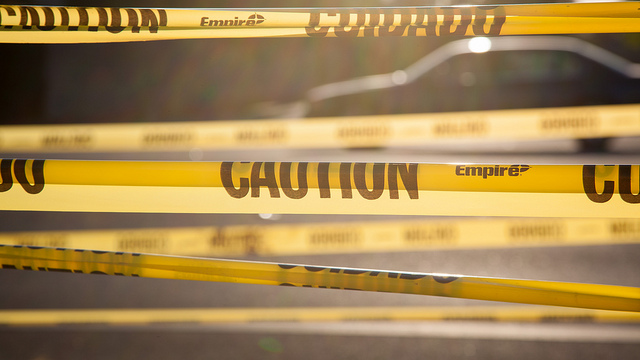
\includegraphics[width=16cm]{figs/caution.jpg}}
\begin{frame}
\frametitle{Limitations}
\begin{columns}[T]
    \begin{column}{0.8\textwidth}
     \begin{block}{Teachers should not rely exclusively on Dr. Scratch}
\begin{itemize}
  \item Fundamental CT skills not assessed: debugging and remixing.
  \item Functionality or creativity not evaluated.
  \item Portfolio analysis would be more accurate.
\end{itemize}
    \end{block}
    \end{column}
  \end{columns}
\vspace{\baselineskip}
\vspace{\baselineskip}
\hfill{\Tiny Background picture:  Robert Couse-Baker}
\end{frame}

\usebackgroundtemplate{}

%--------------------------------------------------------
%\usebackgroundtemplate{
\includegraphics[width=13cm]{figs/take-away.jpg}}
% background: http://2.bp.blogspot.com/-78Eh4TBpdtU/UPw7ULV73PI/AAAAAAAAHAE/6DQfvPNCo-Y/s1600/8723052-stylized-red-stamp-showing-the-term-take-away-all-on-white-background.jpg
\usebackgroundtemplate{
\includegraphics[width=13cm]{figs/future.png}}

\begin{frame}
\frametitle{Future Work}

\begin{enumerate}
  \item User accounts
  \item Teacher dashboard
  \item Organization dashboard
\end{enumerate}
\vspace{\baselineskip}
\vspace{\baselineskip}
\hfill{\Tiny Background picture: Simon Cunningham }

\end{frame}

\usebackgroundtemplate{}
%--------------------------------------------------------
\usebackgroundtemplate{
\includegraphics[width=13cm]{figs/books.jpg}}
% http://www.aspa-usa.org/wp-content/uploads/2015/06/books.jpg
\begin{frame}
\frametitle{Learn more}
\begin{center}
\begin{columns}[T]
    \begin{column}{1\textwidth}
     \begin{block}{Some references}
       \begin{itemize}
	 \item Automatic detection of bad programming habits in scratch: a preliminary study
	 \item Dr. Scratch: automatic analysis of Scratch projects to assess and foster computational thinking
	 \item Comparing computational thinking development assessment scores with software complexity metrics
	 \item Computational thinking test: design guidelines and content validation
       \end{itemize}
    \end{block}
    \end{column}
  \end{columns}
\end{center}
\end{frame}

\usebackgroundtemplate{}

%--------------------------------------------------------
%\begin{frame}
%\frametitle{GSyC/LibreSoft}

%\begin{figure}[t!]
%\begin{center}
%\includegraphics[width=11cm]{figs/libresoft.jpg}
%\end{center}
%\label{fig:libresoft}
%\end{figure}

%\begin{center}
%The GSyC/LibreSoft research team at URJC (Madrid).
%\end{center}

%\end{frame}

%--------------------------------------------------------
%\begin{frame}
%\frametitle{Our work at GSyC/LibreSoft}

%\begin{figure}[t!]
%\begin{center}
%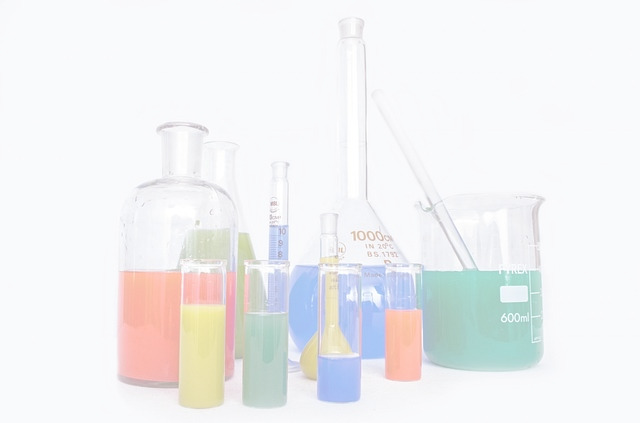
\includegraphics[width=2.5cm]{figs/research}
% http://www.memphis.edu/crow/images/research_2.jpg
%\hspace{0.1cm}
%\includegraphics[width=2.5cm]{figs/teaching}
% http://2.bp.blogspot.com/_uxgwfriLwSo/TOWDr8IjaLI/AAAAAAAABLM/d7H-G5jIq-c/s1600/teaching.gif
%\hspace{0.1cm}
%\includegraphics[width=2.5cm]{figs/development}
% http://www.vidadigitalradio.com/wp-content/uploads/2009/04/hackers_cartoons.jpg
%\hspace{0.1cm}
%\includegraphics[width=2.5cm]{figs/promotion}
% http://bloggeate.com/wp-content/uploads/2011/04/como-promocionar-tu-blog.jpg
%\end{center}
%\label{fig:whatwedo}
%\end{figure}

%\begin{center}
%GSyC/LibreSoft's tasks: research, teaching, development, promotion of free software.

%\end{center}
%\end{frame}

\usebackgroundtemplate{}

%--------------------------------------------------------
\frame{
\maketitle
\begin{center}

\includegraphics[width=2cm]{format/libresoft-logo}
\hspace{0.5cm}

\includegraphics[width=5cm]{format/gsyc-urjc}
\vspace{0.5cm}

\includegraphics[width=3cm]{format/emadrid.png}
\end{center}
}

\end{document}
